\documentclass[notes,blackandwhite,mathsans]{beamer}

\usepackage{amsmath}
\usepackage{amssymb}
\usepackage{graphicx}
\usepackage{fancybox}
\usepackage{booktabs}
\usepackage{multirow,pxfonts}
\usepackage{cmbright}
\usepackage{color}
\usepackage{xcolor}
\usepackage{changepage}

\usepackage[T1]{fontenc}
\fontencoding{T1}  
\usepackage[utf8]{inputenc}


\usefonttheme{default}
\setbeamercovered{invisible}
\beamertemplatenavigationsymbolsempty

\makeatletter
\setbeamertemplate{footline}
{
  \leavevmode
  \hbox{
  \begin{beamercolorbox}[wd=0.97\paperwidth,ht=2.25ex,dp=2ex,right]{}
{\color{mcxs3} \insertframenumber{} / \inserttotalframenumber}
  \end{beamercolorbox}}%
}


\definecolor{mcxs1}{HTML}{05386B}
\definecolor{mcxs2}{HTML}{379683}
\definecolor{mcxs3}{HTML}{5CDB95}
\definecolor{mcxs4}{HTML}{8EE4AF}
\definecolor{mcxs5}{HTML}{EDF5E1}
\setbeamercolor{frametitle}{fg=mcxs2}
\AtBeginDocument{\color{mcxs1}}

%\setbeamercolor{itemize text}{fg=mcxs5}
\setbeamercolor{itemize item}{fg=mcxs1}
\setbeamercolor{itemize subitem}{fg=mcxs2}
\setbeamercolor{enumerate item}{fg=mcxs1}
\setbeamercolor{description item}{fg=mcxs1}

%\setbeamertemplate{itemize item}[triangle]
%\setbeamertemplate{itemize subitem}[circle]






\begin{document}
%\fontfamily{pag}\selectfont
%\setbeamerfont{title}{family=\fontfamily{pag}\selectfont}
%\setbeamerfont{frametitle}{family=\fontfamily{pag}\selectfont}
%\setbeamerfont{framesubtitle}{family=\fontfamily{pag}\selectfont}




\begin{frame}
\centering
\includegraphics[scale=1.87]{mcxs.png}
\end{frame}




{\setbeamercolor{background canvas}{bg=mcxs2}
\begin{frame}

\vspace{1cm}
\begin{tabular}{rl}
&\textbf{\LARGE\color{mcxs1} Macroeconometrics}\\[6ex]
\textbf{\color{mcxs3}\Large Lecture 1}&\textbf{\Large\color{mcxs5}What's macroeconometrics?}\\[19ex]
&\textbf{\color{mcxs1} Tomasz Wo\'zniak}\\[1ex]
&{\small\color{mcxs5} Department of Economics}\\
&{\small\color{mcxs5}University of Melbourne}
\end{tabular}

\end{frame}
}






\begin{frame}{Tomasz Wo\'zniak - short CV}

\textbf{Lived in.}\\
\hspace{0.3cm}{\small Inowroc\l{}aw{\color{mcxs3}, Poland }\\
\hspace{0.3cm}Krak\'ow{\color{mcxs3}, Poland }\\
\hspace{0.3cm}{\color{mcxs2}Firenze}{\color{mcxs3}, Italy }\\
\hspace{0.3cm}Melbourne{\color{mcxs3}, Australia} \\}

\vspace{1cm}\textbf{Education.}\\
{\small {\color{mcxs3}Ph.D. in} {\color{mcxs2} Economics} {\color{mcxs3} at the }European University Institute\\
{\color{mcxs3}M.Res. in Economics at the }European University Institute \\
{\color{mcxs3}M.S. in }IT and Econometrics {\color{mcxs3} at the} {\color{mcxs2} Cracow University of Economics} \\}


\end{frame}


{\setbeamercolor{background canvas}{bg=mcxs5}
\begin{frame}{Tomasz Wo\'zniak - short CV}

\textbf{Research Interests.}\\
\hspace{0.3cm}{\small {\color{mcxs2}Econometrics}\\
\hspace{0.3cm}{\color{mcxs2}Multivariate} {\color{mcxs1}Time Series Analysis}\\
\hspace{0.3cm}\textbf{Bayesian Inference} \\
\hspace{0.3cm}{\color{mcxs2}Economic Forecasting} \\
\hspace{0.3cm}Causality {\color{mcxs2} Analysis}}\\




\vspace{0.5cm}\textbf{Topics I worked on.}\\[0.5ex]
{\small
Granger causality for time-varying volatility \\
{\color{mcxs2}how risk associated with one financial asset transmits to another financial asset's risk}\\[1.5ex]
Heteroskedastic models for monetary policy \\
{\color{mcxs2}how to use volatility of variables to estimate the effect of monetary policy on the real economy more precisely }\\[1.5ex]
\texttt{bsvars}: an \textbf{R} package for structural analyses for economics and finance \\
{\color{mcxs2}provides tools for estimation, structural and predictive analyses }
}
\end{frame}
}




{\setbeamercolor{background canvas}{bg=mcxs2}
\begin{frame}

\bigskip\textbf{\color{mcxs3}What's macroeconometrics?}

\bigskip\textbf{\color{mcxs3}Organization of the subject}

\bigskip\textbf{\color{mcxs1}Research project}

\bigskip\textbf{\color{mcxs3}Models we are working with}

\end{frame}
}








{\setbeamercolor{background canvas}{bg=mcxs2}
\begin{frame}

\begin{adjustwidth}{-0.5cm}{0cm}
%\FlushLeft
\vspace{8.3cm}\Large
\textbf{{\color{mcxs3}What's} {\color{mcxs1}macroeconometrics?}}
\end{adjustwidth}

\end{frame}
}






\begin{frame}{\color{mcxs2}Macroeconometrics}

Macroeconometrics focuses on developing methodology for empirical macroeconomic research.

\bigskip Its main objectives include 
\begin{itemize}
\item {\color{mcxs1}verification of economic theories}
\item {\color{mcxs1}forecasting future developments of essential variables}
\item {\color{mcxs1}providing analyses for data-driven decision-making at governing institutions and their stakeholders}
\end{itemize}

\bigskip It uses dedicated econometric models and procedures that determine the feasibility, robustness, and reliability of the applied research.

\end{frame}



{\setbeamercolor{background canvas}{bg=mcxs5}
\begin{frame}{\color{mcxs2}Macroeconometrics}

The characterization of econometric modeling includes

\smallskip
\begin{itemize}
\item {\color{mcxs1}System modeling} {\color{mcxs2}of many variables in one model}
\item {\color{mcxs1}Identification} {\color{mcxs2}of economically interpretable objects of interest}
\item {\color{mcxs1}Incorporation of economic theory assumptions} {\color{mcxs2}into econometric model specifications}
\item {\color{mcxs1}Efficient extraction of information} {\color{mcxs2}from the data implying e.g. modeling unit-root nonstationary variables}
\end{itemize}
\end{frame}
}



{\setbeamercolor{background canvas}{bg=mcxs4}
\begin{frame}{\color{mcxs1}Macroeconometrics}

Macroeconometrics develops dedicated econometric models and procedures that are data, application, and objective-specific.

\bigskip The development of these methods makes the empirical research possible and reliable.
 
\bigskip Macroeconometrics as a field became highly technical and heavily computational.

\end{frame}
}





\begin{frame}

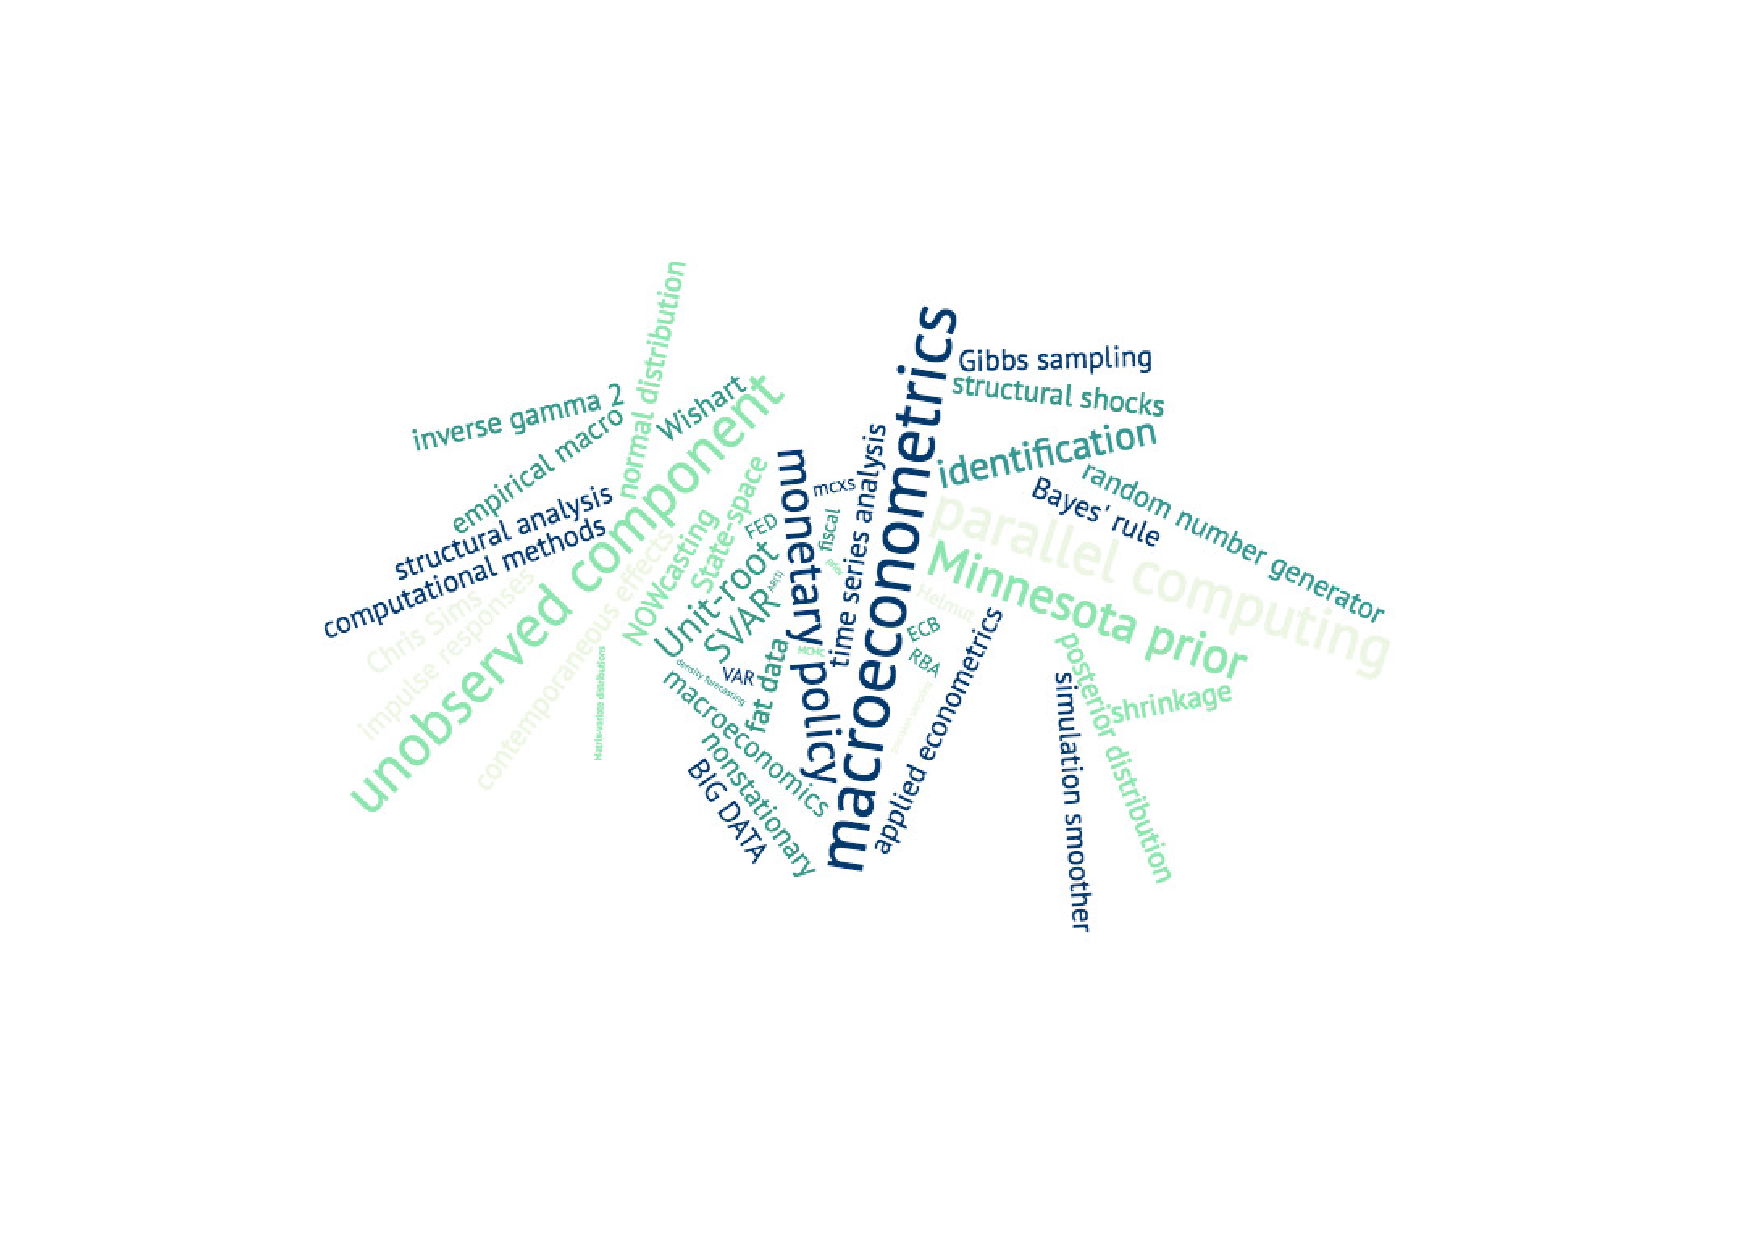
\includegraphics[scale=0.65, trim= 6cm 0cm 0cm 3cm]{grphs/mcxs-wordcloud4.pdf}

\end{frame}




{\setbeamercolor{background canvas}{bg=mcxs4}
\begin{frame}{\color{mcxs1}Macroeconometrics}

\bigskip This subject prepares the students to develop their own methods which requires:

\begin{itemize}
\item {\color{mcxs1}knowing the models} {\color{mcxs2}and their properties}
\item {\color{mcxs1}deriving} {\color{mcxs2}estimation procedures}
\item {\color{mcxs1}writing computer programs} {\color{mcxs2}for these procedures and computation of interpretable values}
\item {\color{mcxs1}employing} {\color{mcxs2}these programs for data analysis}
\end{itemize}

\end{frame}
}










{\setbeamercolor{background canvas}{bg=mcxs3}
\begin{frame}

\begin{adjustwidth}{-0.5cm}{0cm}
%\FlushLeft
\vspace{8.3cm}\Large
\textbf{{\color{mcxs2}Organisation} {\color{mcxs1}of the subject}}
\end{adjustwidth}

\end{frame}
}




\begin{frame}
\frametitle{Contact Info}

\hspace{0.3cm}University of Melbourne \\
\hspace{0.3cm}{\color{mcxs3}Faculty of Business and Economics} \\
\hspace{0.3cm}{\color{mcxs3}Department of Economics} 


\vspace{0.5cm}
\hspace{0.3cm}{\color{mcxs3}email:} \href{mailto:tomasz.wozniak@unimelb.edu.au}{tomasz.wozniak@unimelb.edu.au}\\
\hspace{0.3cm}{\color{mcxs3}website:} {\color{mcxs2}\href{https://github.com/donotdespair}{github.com/donotdespair}}\\

\vspace{0.5cm}
\hspace{0.3cm}{\color{mcxs3}Office No.:} 350{\color{mcxs3}, FBE building}

\end{frame}



\begin{frame}{Lectures}

\textbf{Lectures.}

\smallskip In-person active learning sessions are scheduled on:

\smallskip
\hspace{0.3cm}{\color{mcxs2} Wednesdays} 5:45 – 7:15 pm, FBE 221 (Theatre 4) \\
\hspace{0.3cm}{\color{mcxs2}Thursdays}  3:15 – 4:45 pm, FBE 211 (Theatre 2)

\smallskip Attendance is monitored

\bigskip\textbf{Consultations.}


\smallskip
\hspace{0.3cm}{\color{mcxs2}Wednesdays} 4:30--5:30 pm {\color{mcxs2} FBE 350}


\end{frame}





\begin{frame}
\frametitle{Assessment}

\begin{center}
\begin{tabular}{ l l l }
\toprule 
Week & Task & Grade \\[1ex]
\midrule
4 & \textbf{Test 1:} Concepts and Tools & 10\% \\ [1ex]
5 & \textbf{RP1:} question, data, model, hypothesis & 10\% \\[1ex]
6 & \textbf{Test 2:} Bayesian Estimation & 10\% \\[1ex]
8 & \textbf{RP2:} estimation procedure and algorithm & 10\% \\
10 & \textbf{RP3:} empirical analysis & 10\% \\[1ex]
4--10 & Learning repository contribution & 10\% \\ [1ex]
11 & \textbf{RP Presentation} &  10\% \\[1ex]
12+ & \textbf{RP Final report} & 30\%   \\[1ex]
\bottomrule
\end{tabular}

\smallskip\noindent \textbf{RP} stands for \textbf{R}esearch \textbf{P}roject
\end{center}

\end{frame}



\begin{frame}{Learning outcomes}

\textbf{LO1:} Develop original econometric methodology for applied macroeconomic analyses\\[1ex]
\textbf{LO2:} Propose econometric techniques and models to verify hypotheses that inform fiscal or monetary policy\\[1ex]
\textbf{LO3:} Derive Bayesian estimation procedure for the newly proposed macroeconometric model\\[1ex]
\textbf{LO4:} Write computer programs in R that implement the derived estimation procedure\\[1ex]
\textbf{LO5:} Apply the computer program in the forecasting or structural analyses of Australian macroeconomic data\\[1ex]
\textbf{LO6:} Transparently create econometric data analysis using the newly proposed methodology in a fully reproducible report developed collaboratively

\end{frame}




\begin{frame}{Generic skills}

\textbf{GS1:} Obtain and format data from the original sources in an automated workflow\\[1ex]
\textbf{GS2:} Document the essential data properties and incorporate them in the econometric modelling\\[1ex]
\textbf{GS3:} Handle statistical distributions of parameters and forecasted values to make the econometric analysis feasible\\[1ex]
\textbf{GS4:} Apply linear algebra operations and basic statistical theory to facilitate model estimation, hypothesis verification, and reliable forecasting\\[1ex]
\textbf{GS5:} Create visualisations of data and estimation results that inform economic interpretations \\[1ex]

\end{frame}



\begin{frame}{Generic skills}

\textbf{GS6:} Use functional programming to implement econometric procedures\\[1ex]
\textbf{GS7:} Propose economic interpretations based on the empirical evidence\\[1ex]
\textbf{GS8:} Obtaining, providing, and implementing constructive and actionable feedback\\[1ex]
\textbf{GS9:} Managing a programming and data analysis project using git and GitHub\\[1ex]
\textbf{GS10:} Communicating research outcomes in plain language and using visualisations

\end{frame}







\begin{frame}
\frametitle{Syllabus}

\begin{center}
\begin{tabular}{ c l}
\toprule 
Lecture & Topic \\
\midrule
\multicolumn{2}{c}{\textbf{Concepts and Tools}}\\
1  & {\color{mcxs2}What's macroeconometrics?} \\
2  & {\color{mcxs2}Maximum likelihood estimation}  \\
3  & {\color{mcxs1}Bayesian estimation} \\
4  & {\color{mcxs2}Numerical optimization and integration} \\
5  & {\color{mcxs2}Understanding unit-rooters} \\
6  & {\color{mcxs1}Macroeconometric research themes} \\[1ex]\bottomrule
\end{tabular}
\end{center}
\end{frame}


\begin{frame}
\frametitle{Syllabus}

\begin{center}
\begin{tabular}{ c l}
\toprule 
Lecture & Topic \\
\midrule
\multicolumn{2}{c}{\textbf{Macroeconomic Forecasting with Fat Data}}\\
7  & Vector Autoregressions \\
8  & {\color{mcxs2}Large Bayesian VARs} \\
9  & {\color{mcxs2}Forecasting with Bayesian VARs} \\
10  & {\color{mcxs2}Forecasting with Large Bayesian VARs} \\[1ex]
\bottomrule
\end{tabular}
\end{center}

\end{frame}


\begin{frame}
\frametitle{Syllabus}
\small
\begin{center}
\begin{tabular}{ c l}
\toprule 
Lecture & Topic \\
\midrule
\multicolumn{2}{c}{\textbf{Modeling Effects of Monetary Policy}}\\
11  & {\color{mcxs2}Structural VAR} models \\
12  & {\color{mcxs2}Structural VAR} tools \\
13  & {\color{mcxs2}Bayesian estimation  of Structural VARs} \\
14  & {\color{mcxs2}Modeling effects of monetary policy} \\[1ex]
\bottomrule
\end{tabular}
\end{center}

\end{frame}

\begin{frame}
\frametitle{Syllabus}

\begin{center}
\begin{tabular}{ c l}
\toprule 
Lecture & Topic \\
\midrule
\multicolumn{2}{c}{\textbf{Modeling Trend Inflation}}\\
15  & {\color{mcxs2}Unobserved Component models} \\
16  & {\color{mcxs2}Bayesian estimation using simulation smoother} \\
17  & {\color{mcxs2}Modeling trend inflation} \\[1ex]
\multicolumn{2}{c}{\textbf{Modeling Conditional Heteroskedasticity}}\\
18 & {\color{mcxs2}Stochastic Volatility models} \\
19  & {\color{mcxs2}Bayesian estimation using auxiliary mixtures} \\[1ex]
\multicolumn{2}{c}{\textbf{Topics in Climate Change}}\\
20  & {\color{mcxs2}Forecasting CO$_2$ Emissions for the 21st Century} \\[1ex]
\bottomrule
\end{tabular}
\end{center}
\end{frame}



\begin{frame}
\frametitle{Syllabus}

\begin{center}
\begin{tabular}{ c l}
\toprule 
Lecture & Topic \\
\midrule
\multicolumn{2}{c}{\textbf{Research Project Presentations}}\\
21  & {\color{mcxs2}Student Presentations} \\
22  & {\color{mcxs2}Student Presentations} \\[1ex]
\multicolumn{2}{c}{\textbf{Lecturer's Research Presentation}}\\
23  & {\color{mcxs2}Robust macroeceonometric modelling}\\
24  & {\color{mcxs2}\texttt{bsvars} package presentation} \\[1ex]
\bottomrule
\end{tabular}
\end{center}
\end{frame}








\begin{frame}
\frametitle{Introduction to R}

\noindent The objective of the complementary four sessions is to facilitate the beginning of working with R. 

\bigskip\noindent\textbf{Session 1: {\color{mcxs2}Introduction to R}}

\bigskip\noindent\textbf{Session 2: {\color{mcxs1}Basic programing in R}}

\bigskip\noindent\textbf{Session 3: {\color{mcxs2}Numerical integration}}

\bigskip\noindent\textbf{Session 4: {\color{mcxs2}Numerical optimization}}


\bigskip\noindent\textbf{Session 5: {\color{mcxs2}Quarto documents}}

\bigskip\noindent\textbf{Session 6: {\color{mcxs2}Project development with git and GitHub}}

\bigskip\noindent\textbf{Session 7: {\color{mcxs2}Working with template repository on GitHub}}

\end{frame}





{\setbeamercolor{background canvas}{bg=mcxs3}
\begin{frame}

\begin{adjustwidth}{-0.5cm}{0cm}
%\FlushLeft
\vspace{8.3cm}\Large
\textbf{{\color{mcxs2}Research} {\color{mcxs1}project}}
\end{adjustwidth}

\end{frame}
}





\begin{frame}
\frametitle{Research project}

\begin{center}
\begin{tabular}{ l l l }
\toprule 
Week & Task & Grade \\[1ex]
\midrule
5 & \textbf{RP1:} question, data, model, hypothesis & 10\% \\[1ex]
8 & \textbf{RP2:} estimation procedure and algorithm & 10\% \\[1ex]
10 & \textbf{RP3:} empirical analysis & 10\% \\[1ex]
11 & \textbf{RP Presentation} &  10\% \\[1ex]
12+ & \textbf{RP Final report} & 30\%   \\[1ex]
\bottomrule
\end{tabular}

\end{center}

\end{frame}




\begin{frame}{Research project}

\textbf{The report includes:}
\begin{itemize}
\smallskip\item {\color{mcxs1}a proposal of an original model} {\color{mcxs2}and a hypothesis to be verified}

\item {\color{mcxs1}derivation and coding} {\color{mcxs2}of the Bayesian estimation procedure}

\item {\color{mcxs1}empirical investigation} {\color{mcxs2}answering the proposed hypothesis}
\end{itemize}


\bigskip\textbf{Submission format.}
\begin{itemize}
\smallskip\item {\color{mcxs1}a fully reproducible report} {\color{mcxs2}generated with \textbf{Quarto}}

\smallskip\item {\color{mcxs1}the report is a website} {\color{mcxs2}hosted on \textbf{GitHub}}

\smallskip\item {\color{mcxs1}the project is developed collaboratively} {\color{mcxs2}using management tools \text{git} and \textbf{GitHub}}
\end{itemize}


\end{frame}






\begin{frame}{Research project}

\begin{center}
Each of the \textbf{PR1}--\textbf{PR3} and the \textbf{Presentation} consist of:

\bigskip
\begin{tabular}{ l l l }
\toprule 
Task & Grade \\
\midrule
GitHub and Canvas submission & 8\% \\[1ex]
Providing feedback to your peer & 1\% \\[1ex]
Implementing the feedback in your report & 1\% \\[1ex]
\bottomrule
\end{tabular}

\end{center}

\end{frame}







{\setbeamercolor{background canvas}{bg=mcxs2}
\begin{frame}

\begin{adjustwidth}{-0.5cm}{0cm}
%\FlushLeft
\vspace{8.3cm}\Large
\textbf{{\color{mcxs3}Models } {\color{mcxs1}we are working with}}
\end{adjustwidth}

\end{frame}
}




\begin{frame}{Models we are working with}

\textbf{Vector Autoregressions.}
\begin{align*}
y_t &= A_1 y_{t-1} + \dots + A_p y_{t-p}  + \mu_0 + \epsilon_t\\[1ex]
\epsilon_t|Y_{t-1} &\sim iid\left(\mathbf{0}_N,\Sigma\right)\\
\end{align*}

\begin{description}
\item[System modelling] {\color{mcxs2}-- all variables are endogenous} 
\item[Dynamics] {\color{mcxs2}-- captures system dynamics of the variables} 
\item[Forecasting] {\color{mcxs2}-- a go to model for predictive applications} 
\item[Extensions] {\color{mcxs2} capturing important data features improve forecasting precision}
\end{description}
\end{frame}




\begin{frame}{Models we are working with}

\textbf{Structural Vector Autoregressions.}
\begin{align*}
y_t &= A_1 y_{t-1} + \dots + A_p y_{t-p}  + \mu_0 + \epsilon_t\\[1ex]
B\epsilon_t &= u_t \\[1ex]
u_t|Y_{t-1} &\sim iid\left(\mathbf{0}_N,I_N\right)\\
\end{align*}

\begin{description}
\item[Structural] {\color{mcxs2}relationships are explicitly modelled} 
\item[Economic theory] {\color{mcxs2}informs identification of structural shocks} 
\item[Dynamic causal effects] {\color{mcxs2}can be estimated and interpeted} 
\item[Policy decision-making] {\color{mcxs2}is based on evidence provided by SVARs}
\end{description}
\end{frame}




\begin{frame}{Models we are working with}

\textbf{Unobserved Component Models.}
\begin{align*}
y_t &= \tau_t + \epsilon_t\\[1ex]
\tau_t &= \mu + \tau_{t-1} + \eta_t \\[1ex]
\epsilon_t &= \alpha_1 \epsilon_{t-1} + \dots +  \alpha_p \epsilon_{t-p} + e_t \\[1ex]
\eta_t|Y_{t-1} &\sim iid\mathcal{N}\left(0,\sigma_\eta^2\right)\\[1ex]
e_t |Y_{t-1} &\sim iid\mathcal{N}\left(0,\sigma_e^2\right)
\end{align*}

\begin{description}
\item[Trend and cycle] {\color{mcxs2}decomposition of a variable} 
\item[Long-run trend] {\color{mcxs2}is highly-persistent} 
\item[Oscillating cycle] {\color{mcxs2}captures short-term dynamics} 
\item[Inflation trend analysis] {\color{mcxs2}and output gap estimation are the main applications}
\end{description}
\end{frame}




{\setbeamercolor{background canvas}{bg=mcxs4}
\begin{frame}{}

\bigskip
\begin{center}
\LARGE\textbf{Macroeconometrics means cooperation!}
\end{center}



\end{frame}
}





\end{document} 